\section{Przegląd komercyjnych rozwiązań TRNG}\label{sec:przeglad-komercyjnych-rozwiazan-trng}

Komercyjne rozwiązania bazują na przeróżnych źródłach entropii,
najczęściej nie na dostarczanych przez użytkownika, aby wykluczyć możliwość ingerencji i ograniczyć przewidywalność, a na całkowicie niezależnych.
Najpopularniejszym medialnie RNG jest LavaRand~\cite{cloudflare_lavarand}, który inspirowany był podobnym systemem,
zbudowanym i opatentowanym przez Silicon Graphics~\cite{SiliconGraphics}.
LavaRand jest dzisiaj jedynie dodatkowym zabezpieczeniem firmy Cloudflare,
na wypadek gdyby ich konwencjonalne źródła entropii okazały się niewystarczające.
Wciąż jednak pozostaje inspirującym przykładem do szukania losowości w zjawiskach otaczających ludzi w codziennym życiu.

\begin{figure}[h]
    \centering
    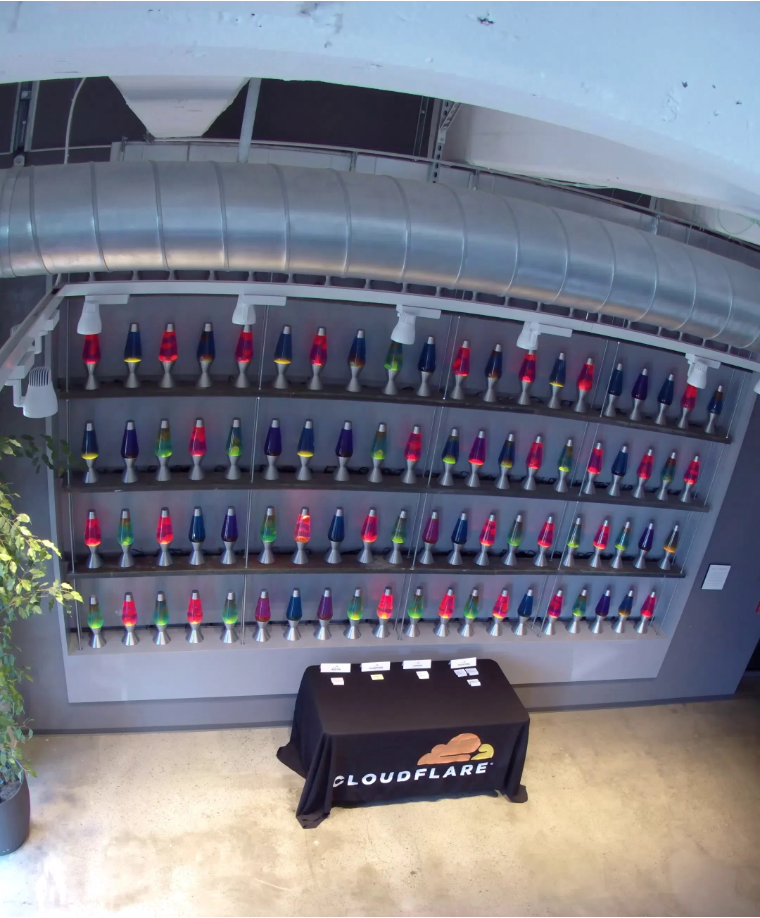
\includegraphics[width=0.4\linewidth]{chapters/02-teoria/figures/lavarandCamera}
    \caption{Widok z kamery w biurze Cloudflare~\cite{cloudflare_lavarand}.}
    \label{fig:lavarand}
\end{figure}

Silicon Graphics oferuje użytkownikom dostęp do generatora liczb losowych w chmurze, który jest wykorzystywany
m.in. do tworzenia kluczy kryptograficznych oraz w innych zastosowaniach wymagających silnych zabezpieczeń.
Dzięki wykorzystaniu globalnej infrastruktury Cloudflare, generowane liczby losowe są
szeroko dostępne i charakteryzują się dużą niezawodnością oraz odpornością na ataki.

W ostatnich latach pojawiły się także inne rozwiązania chmurowe, które umożliwiają generowanie liczb losowych w czasie rzeczywistym bez potrzeby posiadania własnego sprzętu,
za to na przykład za pośrednictwem API takiego jak \textit{drand}~\cite{drand_documentation}.
Przykładem takiego rozwiązania jest Cloudflare – firma specjalizująca się w dostarczaniu usług związanych z bezpieczeństwem sieciowym.
Na swoim blogu Cloudflare przedstawia zaawansowane metody generowania liczb losowych, które są wykorzystywane w ich systemach~\cite{cloudflare_league_of_entropy}.
Dodatkowo wspomniana firma korzysta również z technologii opartych na zjawiskach fizycznych, takich jak rozpad radioaktywnego uranu,
trójstopniowego wahadła, czy „Entropy Wall”, która pobiera entropię z kamery
ustawionej na ścianę lamp lawowych, pokazanej na rys.~\ref{fig:lavarand}.
Te prawdziwie losowe wartości zostają potem użyte jako ziarno dla generatorów pseudolosowych.
Tego typu rozwiązania pozwalają na szybkie i bezpieczne generowanie liczb losowych w skali globalnej, zapewniając jednocześnie wysoki poziom ochrony przed atakami.

\subsection{Rozwiązania sprzętowe}\label{subsec:rozwiazania-sprzetowe}
Wiodącymi producentami komercyjnych rozwiązań sprzętowych są firmy takie jak
ID Quantique~\cite{IDQ}, Microchip Technology~\cite{MicrochipTechnology} i Semtech~\cite{Semtech},
które oferują zaawansowane urządzenia bazujące na TRNG.
Produkty te zapewniają wysoki poziom bezpieczeństwa i są stosowane w wymagających tego aplikacjach,
takich jak bankowość elektroniczna czy systemy wojskowe.

ID Quantique jest jednym z liderów w dziedzinie generatorów liczb losowych opartych na technologii fotoniki i mechanizmach kwantowych.
Firma oferuje urządzenia, które wykorzystują detekcję fotonów w celu generowania liczb losowych.
Dzięki temu rozwiązania ID Quantique charakteryzują się bardzo wysoką jakością losowości,a jednocześnie są odporne na ataki związane z analizą i przewidywaniem generowanych liczb.

Microchip Technology w swojej ofercie posiada różne moduły TRNG, w tym układy scalone,
które generują liczby losowe na podstawie fluktuacji szumów termicznych.
Produkty te znajdują zastosowanie w szerokim zakresie aplikacji, od urządzeń mobilnych po systemy wbudowane.

Semtech natomiast oferuje rozwiązania, które wykorzystują zjawiska losowe
zachodzące w obwodach analogowych do generowania liczb losowych.
Firma ta jest jednym z głównych dostawców układów IoT, które wykorzystują własne generatory TRNG
do generowania wartości losowych w systemach komunikacji bezprzewodowej.


\subsection{Podobne rozwiązania}\label{sec:podobne-rozwiazania}

Szukając dostępnych na rynku TRNG, można znaleźć wiele interesujących projektów. Są to zarówno rozwiązania komercyjne, 
najczęściej produkowane przez firmy wymienione powyżej, jak i otwartoźródłowe. Niewiele z nich jednak jest zbliżonych 
do realizowanego projektu. Wśród znalezionych rozwiązań zaledwie dwa inspirowały się fizycznym rzutem kością.

Pierwszym ze znalezionych rozwiązań był projekt \textit{The Smart Dice Cup}, zrealizowany przez Carstena Magerkurth,
Timo'a Engelke i Carstena Röcker~\cite{SmartDice}.
Jest on inspirowany tradycyjnymi kubkami do gry w kości, przypomina je w swojej konstrukcji i sposobie działania.
Urządzeniem należy potrząsnąć, aby uzyskać losową liczbę.
Wynik takiego „rzutu” pokazywany jest na wyświetlaczu LED, zamontowanym na „pokrywce” urządzenia.
Podstawową różnicą między realizowanym projektem a \textit{The Smart Dice Cup} jest brak wykorzystania prawdziwych
kości w drugim rozwiązaniu.
Zamiast tego wynik jest generowany na podstawie zmiany prędkości, z jaką potrząsane jest urządzenie.

Drugim rozwiązaniem jest urządzenie wykorzystane w eksperymencie opisanym w artykule \textit{Dice thrown by cup and machine in PK tests} autorstwa J. B. Rhine~\cite{betoniarka43}.
Jest on najbardziej zbliżony do przedstawionego w poniższej pracy projektu, ponieważ również wprawia kość w
ruch za pomocą obracającego się mechanicznie pojemnika.
Z racji na dostępne technologie, z którymi pracował J. B. Rhine, odczytywanie wyników musiało odbywać się ręcznie, a nie za pomocą małej kamery i sztucznej inteligencji.
Jednakże, konstrukcja urządzenia jest bardzo podobna do zaprezentowanego w sekcji~\ref{subsec:prototypowanie} pierwszego wariantu robota.